% !TEX root = ../thesis.tex

\todofr{
\begin{itemize}
	\item General reference, say that aim is to be self contained rather than completely general, suggest Brown and Rockafellar for the details.
	\item notations inspired from \citet{wainwright08}
\end{itemize}
}

\subsubsection*{Log partition function and natural parameter space
}
%Following \citet{wainwright08} 
We define the \emph{exponential family} $\mathcal F_\phi(\mathcal X)\subseteq\mathcal P(\mathcal X)$ associated with a sufficient statistic $\phi:\mathcal X\to\R^{d}$ on a set $\mathcal X\subseteq \R^{n}$ as the collection of probability distribution functions indexed by a parameter $\theta\in\R^{d}$ and of the form\add{review notations, stick to theta}
%
\eqa{
	q_\theta(x)&=& \exp\pat{\scal{\theta,\phi(x)}-A(\theta)}
}
%
with respect to a base measure $\nu$ on $\mathcal X$. The \emph{log partition} function $A$ is defined such as to normalise $q_{\theta}$:
%
\eqa{
	A(\theta) &=& \log \int_{\mathcal X} \exp\scal{\theta,\phi(x)}\nudx
.
}
%
The set of \emph{natural parameters} $\Omega \subseteq \mathbb R^{d}$ is defined as the set of parameters $\theta$ such that $A(\theta)$ is bounded (and, therefore, $q_\theta$ is a proper distribution):\add{stuff drawn not from WJ but reference in comment above (spring10)}\check{april16}
\eqa{	\Omega &:=& \{\theta\in\R^{d}\mid A(\theta) \,<\,\infty\}.\label{def:natural} 	}
%
An exponential family is said to be \emph{regular}\margnote{regular fam.} when the corresponding set $\Omega$ is nonempty and open. Additionally, an exponential family is said to be \emph{minimal}\margnote{minimal fam.} provided there does not exist a nonzero vector $a\in\mathbb R^{d}$ such that $\scal{a,\phi(x)}$ is constant $\nu$-almost everywhere. A distribution in a minimal exponential family is therefore one-to-one with its parameter $\theta\in\Omega$. In the rest of this document, we will assume that we are working with a regular and minimal exponential family unless otherwise mentioned.\add{is this ever the case?}\check{april 16}

The log-partition function $A$ is convex on $\Omega$. Indeed, let $\theta_1,\theta_2\in\Omega$ and $\lambda\in[0,1]$, then using H\"older's inequality with parameters $(1-\lambda)\inv$ and $\lambda\inv$, we can write:\footnote{For two real-valued measurable functions $f$ and $g$, H\"older's inequality with parameters $p,q\in[1,\infty]$ states that $\|fg\|_{1}\le \|f\|_{p}\|g\|_{q}$ provided $p\inv+q\inv=1$.}
\eqa{
	\int \exp\scal{(1-\lambda)\theta_1,\phi(x)}\exp\scal{\lambda\theta_2,\phi(x)}\nudx\hspace*{-2cm}&&\nn\\
	 &\le& \exp(A(\theta_1))^{1-\lambda} \exp(A(\theta_2))^{\lambda}.\label{eq:holderlogp}
}
Taking the logarithm of that inequality shows that $A$ is convex on $\Omega$ and therefore that $\Omega$ itself is convex.\check{april 16}\todo{Actually $\Omega$ is the \emph{effective domain} of $A$, Rockafellar p.23}
%
\subsubsection*{Gradient and convex-conjugate of $A$}
In a regular exponential family, it is well known \citep[theorem 2.2]{brown86} that the log-partition function is infinitely continuously differentiable and that its gradient and Hessian are related to the first two moments of the sufficient statistic:\add{make sure the notations are clarified somewhere}
%
\eqa{
	\nabla A(\theta) &=& \E_{q_\theta}[\phi(X)] \nn\\
	\nabla^{2}	A(\theta) &=& \mathbb V_{q_\theta}[\phi(X)].\nn
}
%
An important consequence is that, for a minimal exponential family, the covariance matrix $\V_{q_\theta}[\phi(X)]$ is positive definite which in turns implies that $A$ is strictly convex on $\Omega$. Indeed, take any nonzero vector $a\in\mathbb R^{d}$ then by definition, $\scal{a,\phi(X)}$ cannot be constant $\nu$-almost everywhere so that $\mathbb V_{q_{\theta}}[\scal{a,\phi(X)}] > 0$ for any $\theta\in\Omega$ and therefore:
\eqa{	0 &<& \scal{a ,\mathbb V_{q_{\theta}}[\phi(X)] a}, 	}
so that $\mathbb V_{q_{\theta}}[\phi(X)]$ is positive definite.\check{april 16} 
Let $\mathcal M^{\star}$ denote the image of $\Omega$ under the gradient mapping $\nabla A$ or $\mathcal M^{\star}=\nabla A(\Omega)$. Since $A$ is strictly convex, $\nabla A$ is a strictly monotone map, and it forms a bijection between $\Omega$ and $\mathcal M^{\star}$. Let $\theta^{\star}$ be the image of a point $\mu^{\star}\in\mathcal M^{\star}$ through the inverse map $(\nabla A)\inv$. 
This can be written as
%
\eqa{
	\theta^{\star} &=& \{ \theta\in\Omega \mid \nabla A(\theta)=\mu^{\star}\},\nn\\
	&=& \{ \theta\in\Omega\mid \nabla(A(\theta)-\scal{\theta,\mu^{\star}})=0\}.
}
%
Since $A(\theta)-\scal{\theta,\mu}$ is a strictly convex function in $\theta$, this corresponds to a first-order condition for its minimiser.
\footnote{A first-order condition for a minimiser indicates that for a convex, differentiable function $f$ on a set $\Omega$, $\{x\in\Omega\mid \nabla f(x)=0 \}\subseteq\arg\min_{x}\,\,f(x)$. If there exists a unique point $x^{\star}\in\Omega$ such that $\nabla f(x^{\star})=0$ then it is also the unique minimiser of $f$ and both sets are equal to that point \citep[theorem 27.1]{rockafellar70}. } We can therefore write\check{april 16}
%
\eqa{
	\theta^{\star} &=& \arg\min_{\theta\in\Omega} \quad A(\theta)-\scal{\theta,\mu^{\star}}
}
%
which is related to the convex-conjugate of $A$ on $\mathcal M^{\star}$ defined as
\eqa{
	A^{\star}(\mu) &:=& \max_{\theta\in\Omega}\quad \scal{\theta,\mu} - A(\theta).\label{eq:defconja}
}
Note that $A^{\star}$ is itself a convex function. Using this definition, we have
%
\eqa{	
	A^{\star}(\mu^{\star}) &=& \scal{\theta^{\star},\mu^{\star}}-A(\theta^{\star})	\label{eq:duality1}
}
%
and $(\theta^{\star},\mu^{\star})$ is said to form a \emph{dual pair}. Let us now consider an arbitrary $\theta^{+}\in\Omega\backslash\{\theta^{\star}\}$ and the corresponding $\mu^{+}=\nabla A(\theta^{+})\in\mathcal M^{\star}$. Then, by strict convexity of $A$, we have\check{april 17}
%
\eqa{	
	A(\theta^{\star}) &>& A(\theta^{+}) + \scal{\theta^{\star}-\theta^{+},\mu^{+}}.	
	}
%
Using the duality property \eqref{eq:duality1} and with $\mu^{\star}=\nabla A(\theta^{\star})$, the previous inequality reads
%
\eqa{	
	-A^{\star}(\mu^{\star}) + \scal{\theta^{\star},\mu^{\star}} &>& -A^{\star}(\mu^{+})+\scal{\theta^{+},\mu^{+}} + \scal{\theta^{\star}-\theta^{+},\mu^{+}}.\nn\\
	\Longleftrightarrow	\quad A^{\star}(\mu^{+}) &>& A^{\star}(\mu^{\star}) + \scal{\mu^{+}-\mu^{\star},\theta^{\star}}.
	}
%
Since this inequality holds for any $\mu^{+}\neq \mu^{\star}$, $\theta^{\star}$ is said to be a \emph{subgradient} of $A^{\star}$ at $\mu^{\star}$. Since the mapping $\nabla A$ is one-to-one on $\Omega$, $\theta^{\star}$ is necessarily the only such subgradient. Therefore, $A^{\star}$ is differentiable on $\mathcal M$ \citep[theorem 25.1]{rockafellar70} and $\nabla A^{\star}$ is the inverse mapping of $(\nabla A)\inv$ from $\mathcal M^{\star}$ to $\Omega$. The relationship is illustrated at the \fig{bijOmM} below.

\begin{figure}[!h]
	\center
	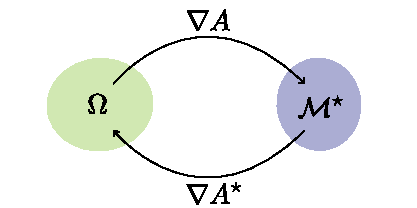
\includegraphics{figures/expf/mapping}
	\caption{\label{bijOmM}Illustration of the bijection between the set of natural parameters $\Omega$ and its image under $\nabla A$, $\mathcal M^{\star}$.}
\end{figure}
%
\subsubsection*{Mean parameter space}
It remains to characterise more precisely the set $\mathcal M^{\star}=\nabla A(\Omega)$. It is a subset of the set of realisable \emph{mean parameters}:\add{notations, set of pdfs in L1}
%
\eqa{
	\mathcal M^{\star} \esp\subseteq\esp \mathcal M &:=& \pab{\mu\in\mathbb R^{d}\mid \exists\, p \in\mathcal P(\mathcal X) \,\,\text{s.t.}\,\, \mu=\E_{p}[\phi(X)] },
}
%
where $\mathcal P(\mathcal X)$ denotes the set of all probability density functions on $\mathcal X$. This space $\mathcal M$ is also known as the \emph{mean parameter space}. It is easy to see that it is convex since $\mathcal P(\mathcal X)$ is trivially convex. More interestingly, it can be shown that, for a minimal exponential family, $\mathcal M^{\star}$ is, in fact, the interior of $\mathcal M$ \citep[theorem 3.3]{wainwright08}. Note that, since the interior of a convex set is necessarily convex, $\mathcal M^{\star}$ is itself convex. Finally, note that since $\mathcal M^{\star}=\mathrm{int}\,(\mathcal M)$, $A^{\star}$ can be continuously extended on $\mathcal M$ by changing the $\max$ in a $\sup$ in \eqref{eq:defconja}. \check{april 17}In a similar fashion, for a point $\mu\in\mathcal M\backslash \mathcal M^{\star}$, we can consider a sequence of points $\mu_{1},\mu_{2},\dots$ in $\mathcal M^{\star}$ such that $\lim_{i\to\infty}\mu_{i}=\mu$ and identify $\nabla A^{\star}(\mu)$ to $\lim_{i\to\infty}\nabla A^{\star}(\mu_{i})$ by continuity. The extended operator is then defined as a mapping from $\mathcal M$ to $\overline\Omega$, the closure of $\Omega$. 
\add{max/sup in notations?, discussion of boundary of Omega for EP when problem in projecting}\check{april 22}

